\chapter{User Interaction}

In this chapter we will incorporate User Interaction into our game. First, we
will add the player's avatar, the pot, to the game. Then we will be
implementing a drag and drop mechanism that lets the user move that pot in order
to catch objects.

While implementing the drag and drop feature you'll learn how \cocos{}'s touch
system works in detail.

\section{Add the Pot to the Game}
The goal of our game will be to move a pot across the screen and try to catch
food while avoiding catching inedible objects. Before we can
implement the drag and drop mechanism we need to add the pot assets to our game,
we're going to do that in the \SB{} project.

Just as in the game we built in the very first chapter we are going to create an
individual \ccbfile{} for this new entity. That way we can encapsulate its
assets, behavior and animations nicely.

One important aspect of this game is the ability to for objects to fall into
our pot. Since we are building a 2D game we need to fake the conception of depth
in our scene. In \cocos{} we can use the z-order to influence which sprites are
rendered in which order. Using that z-order, and using two assets for to create
the pot, we can make it look like objects drop into the pot:

\begin{figure}[H]
    \centering
    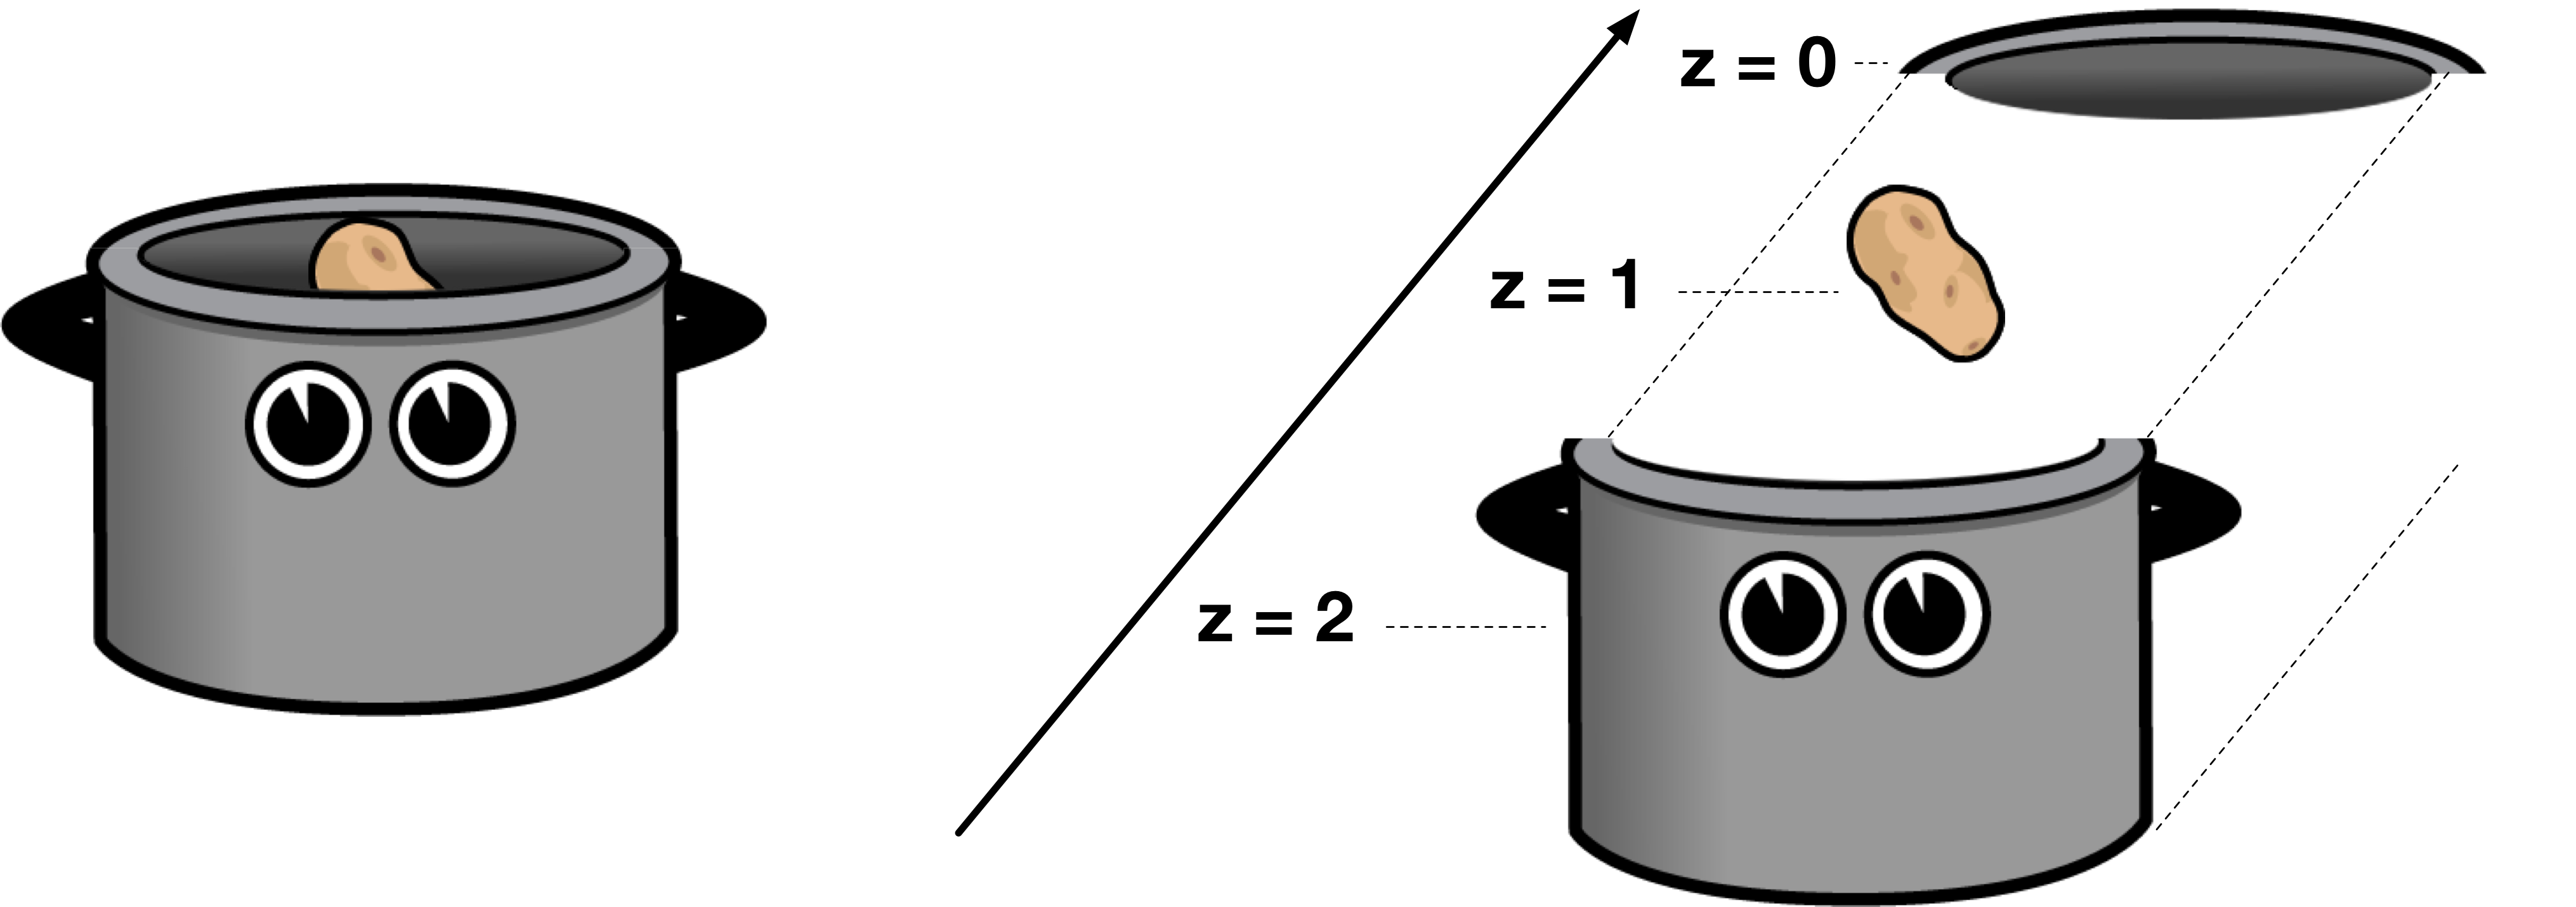
\includegraphics[width=0.9\linewidth]{images/Chapter3/drawing_order.png}
    \caption{Left: Sprites rendered on different layers, Right: How the z-Order
    influences on which layer a sprite is rendered}
\end{figure}

It's essential for this trick to break down the pot into two assets. Such
rendering tricks are very common in 2D games!

\subsection{Setting Up the Pot Assets}
Now that we know which assets we'll use for the pot, let's set up
its \ccbfile{} in \SB{}:
\begin{leftbar}
\begin{enumerate}
  \item Create a new \ccbfile{} of type \textit{Node} and name it
  \textit{Pot.ccb}: \begin{figure}[H]
    \centering
    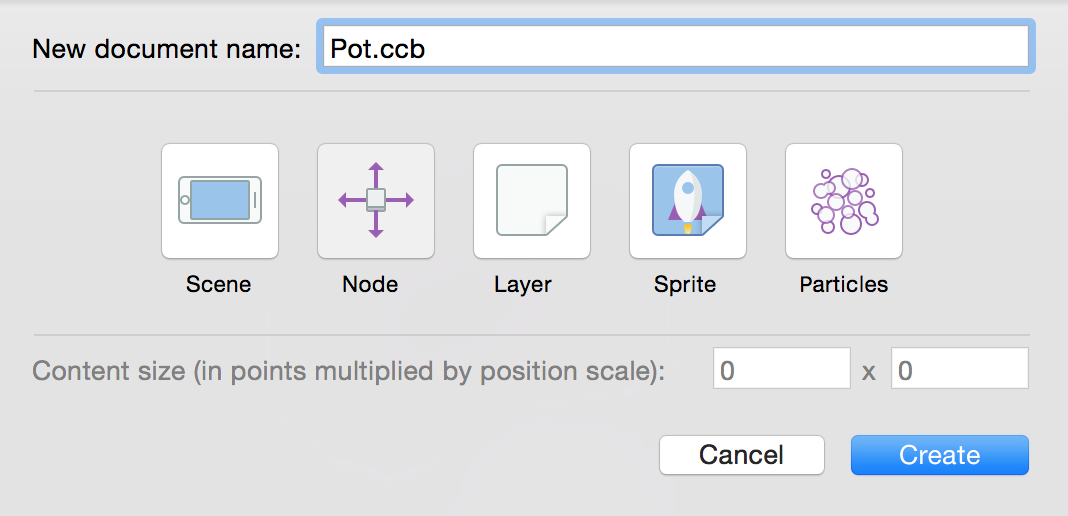
\includegraphics[width=180pt]{images/Chapter3/ccp_pot_file.png}
  \end{figure}
  \item Open the new \filemention{Pot.ccb} file
  \item Drag the \filemention{pot-top} and \filemention{pot-bottom} assets onto
  the root node of that \ccbfile{}: \begin{figure}[H]
    \centering
    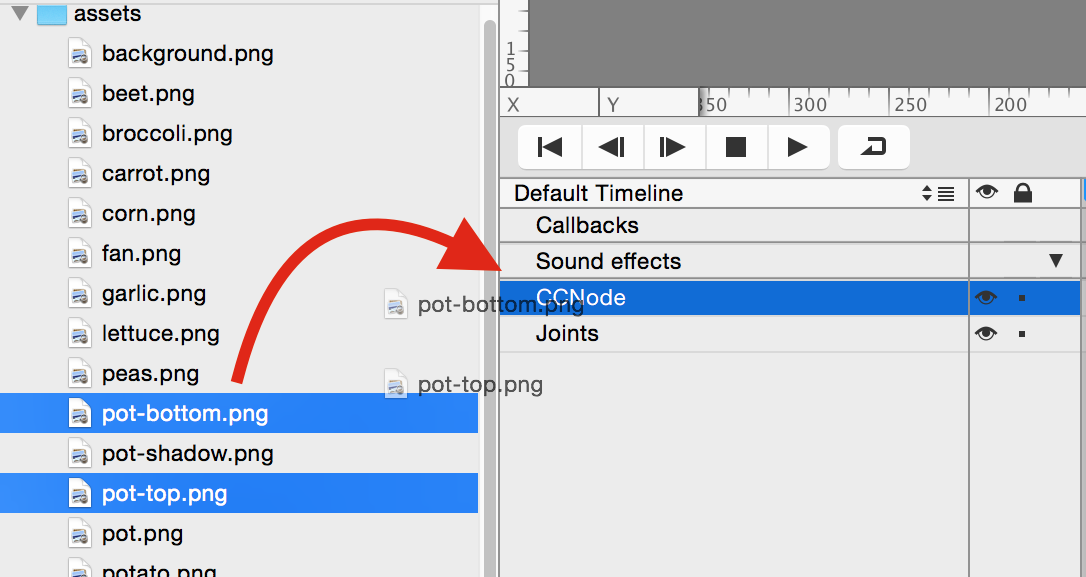
\includegraphics[width=250pt]{images/Chapter3/drag_pot_assets.png}
  \end{figure}
  
  \item Select the root node and set the \textit{Content Size} to (109, 75) and
  the \textit{Anchor Point} to (0.5, 0.5)
  \item Select the \textit{pot-top} sprite from the timeline and set the
  \textit{Position Type} to \textit{Percent of Parent Container}, for both
  \textit{X} and \textit{Y}. Then set the position to \textit{(50, 50)}:
  \begin{figure}[H]
    \centering
    
\includegraphics[width=150pt]{images/Chapter3/pot_top_position.png}
  \end{figure}
  \item Select the \textit{pot-bottom} sprite from the timeline and set up the
  same position as for \textit{pot-top}
  \item Finally, use the shortkey \textit{CMD+S} to save this \ccbfile{}. That
  will prevent a little rendering bug in the next step
\end{enumerate}
\end{leftbar}

The result should be a pot that is centered on stage! You might wonder why we
are setting an explicit size for the root node of \filemention{Pot.ccb}. We do
that because that root node will be used to test against touch positions when we
implement the dragging mechanism. Therefore we want that root node to have the
same dimensions as the pot assets.

In a second we're going to move on and implement the touch handling code. First
however, we need to add the pot that we created to the
\filemention{MainScene.ccb} file. \SB{} allows us to add a \ccbfile{} to other
\ccbfile{} - that's an extremely useful feature as it allows us to reuse
components in different scenes.

We'll also need to set up a code connection, so that we can access the pot
from our codebase when implementing the drag and drop mechanism later on!

\begin{leftbar}
\begin{enumerate}
  \item Open \filemention{MainScene.ccb}
  \item Drag the \filemention{Pot.ccb} file from the left panel onto the root
  node in the timeline of \filemention{MainScene.ccb}:
    \begin{figure}[H]
    \centering
    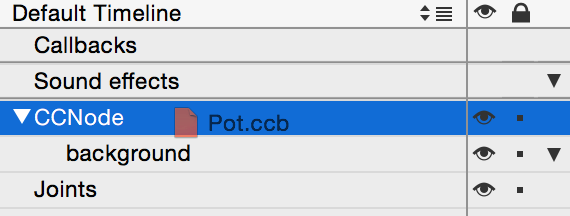
\includegraphics[width=150pt]{images/Chapter3/drag_pot_ccb.png}
  \end{figure}
  \item Set the \textit{Position Type} of the pot to \textit{Percent of parent
  container} for the \textit{X} component
  \item Set the \textit{Position} to \textit{(50, 58)}
  \item Select the pot, open the \textit{Code Connections} tab in the right
  panel and set up a connection to the \textit{Doc root var} named
  \textit{pot}:
  \begin{figure}[H]
    \centering
    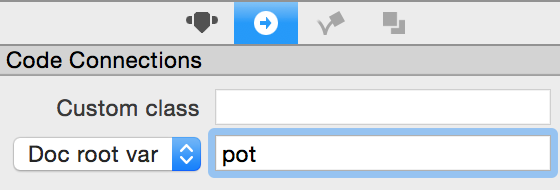
\includegraphics[width=150pt]{images/Chapter3/pot_cc.png}
  \end{figure}
  \item Finally, publish the \SB{} project!
\end{enumerate}
\end{leftbar}

Now we can move to the \xcode{} project to set up the code connection variable
we just defined in \SB{}. Then we're ready to implement the touch handling
code!

\begin{leftbar}
Open \inlinecode{MainScene.swift} and add properties for our code
connection at the top of the class:
\begin{lstlisting}
weak var pot: CCSprite!
\end{lstlisting}
\end{leftbar}
There are three important things to remember about this code connection.

Firstly, all code connections should be marked as \inlinecode{weak}.
\inlinecode{MainScene} has a reference to the pot sprites but does not
\textit{own} them. Instead they are owned by their parent node. For any
references that don't mark an ownership, \inlinecode{weak} should be used. 

Secondly, we always want to declare code connections as \textit{forcefully
unwrapped optionals} as denoted by the bang (!) after the type. Swift
requires that all properties that aren't optionals are either
initialized with a default value or get set to a value in one of the
initializers of the class. That way the compiler can guarantee that these
variables never contain a \inlinecode{nil} value. Code connections however are
set up after the object is initialized (they are guaranteed to be set up
when \inlinecode{didLoadFromCCB} is called on the node), so technically these
should be optional values. Adding a lot of code for \inlinecode{nil} checking
would clutter our classes, that's why we prefer using the bang notation which
basically says: \textit{I am confident that this value will never be nil when I
am trying to access it}. This is true for code connections as we know that
\cocos{} guarantees to have set them up by the time \inlinecode{didLoadFromCCB}
is called.

Lastly, be careful not to mark these variables as \inlinecode{private}.
Otherwise \cocos{} will not have access to them and won't be able to set up the
code connections.

Okay, now we have the basics set up and are ready to dive into the details of
implementing a drag and drop mechanism!

\section{Implement a Drag and Drop Mechanism}
For the very first project in this book we have already implemented a basic
touch mechanism. You should remember that \inlinecode{userInteractionEnabled} is
the property that activates/deactivates touch handling for a node and that
\cocos{} provides four different callbacks for different state transitions in
the lifecycle of a touch. Here's the recap:

\begin{description}
\item[touchBegan:] called when a touch begins
\item[touchMoved:] called when the touch position of a touch changes
\item[touchEnded:] called when a touch ends because the user stops touching the
screen
\item[touchCancelled:] called when a touch is cancelled because user moves touch
outside of the touch area of a node
\end{description}

Knowing that, how can we implement a drag and drop control scheme for our game?
Dragging and dropping includes three different steps:
\begin{enumerate}
  \item Pick up object
  \item Drag object
  \item Drop object
\end{enumerate}

\subsection{Picking Up an Object}
In order to pick up an object we need to detect a user's touch and determine if
the touch is within the boundaries of our object, if that is the case,
we start dragging the object.

First of all, let's turn on user interaction for the \inlinecode{MainScene}
class, so that we receive touch events.

\begin{leftbar}
Add the required line to the \inlinecode{onEnterTransitionDidFinish} method:
\begin{lstlisting}
  override func onEnterTransitionDidFinish() {
    super.onEnterTransitionDidFinish()
    
    (*@\colorbox{light-gray}{userInteractionEnabled = true}@*) 
    
    // spawn objects with defined frequency
    schedule("spawnObject", interval: spawnFrequency)
  }
\end{lstlisting}
\end{leftbar}

Next, we need to add the touch handling method. The touch handling method will
need to check if the touch is within our pot. If that is the case, the method
will need to set a state variable that remembers that we are currently dragging
this object. If the user moves a finger across the screen and we are currently
in object dragging mode, it is important that the object follows the finger of
the user.

\begin{leftbar}
Add this implementation to \inlinecode{MainScene.swift}:
\begin{lstlisting}
  override func touchBegan(touch: CCTouch, withEvent event: CCTouchEvent) {
    if (CGRectContainsPoint(pot.boundingBox(), touch.locationInNode(self))) {
      isDraggingPot = true
      dragTouchOffset = ccpSub(pot.anchorPointInPoints, touch.locationInNode(pot))
    }
  }
\end{lstlisting}
\end{leftbar}

Let's discuss this implementation briefly. You already have seen the usage of 
\linebreak \inlinecode{touch.locationInNode(self)} in the first chapter of this
book, where we briefly discussed touch handling
(\ref{Introduction_FirstTouchHandling}). This method returns the touch position
within a given node. In this specific case we are receiving the touch position
within \inlinecode{MainScene}.

Next, we are using a utility function, \inlinecode{CGRectContainsPoint}, to
check if this touch is within the pot's bounding box.
\inlinecode{CGRectContainsPoint} takes a rectangle as its first argument and a
point as its second. It returns true if the point is within the rectangle.

If the touch position is inside of the pot, we set our state variable,
\inlinecode{isDraggingPot}, to \inlinecode{true}. 

There is one last line that we didn't discuss upfront:
\begin{lstlisting}
dragTouchOffset = ccpSub(pot.anchorPointInPoints, touch.locationInNode(pot))
\end{lstlisting}

In order to drag an object smoothly we need to remember where we touched that
object when starting dragging. Take a look at the following diagram:
\begin{figure}[H]
		\centering
		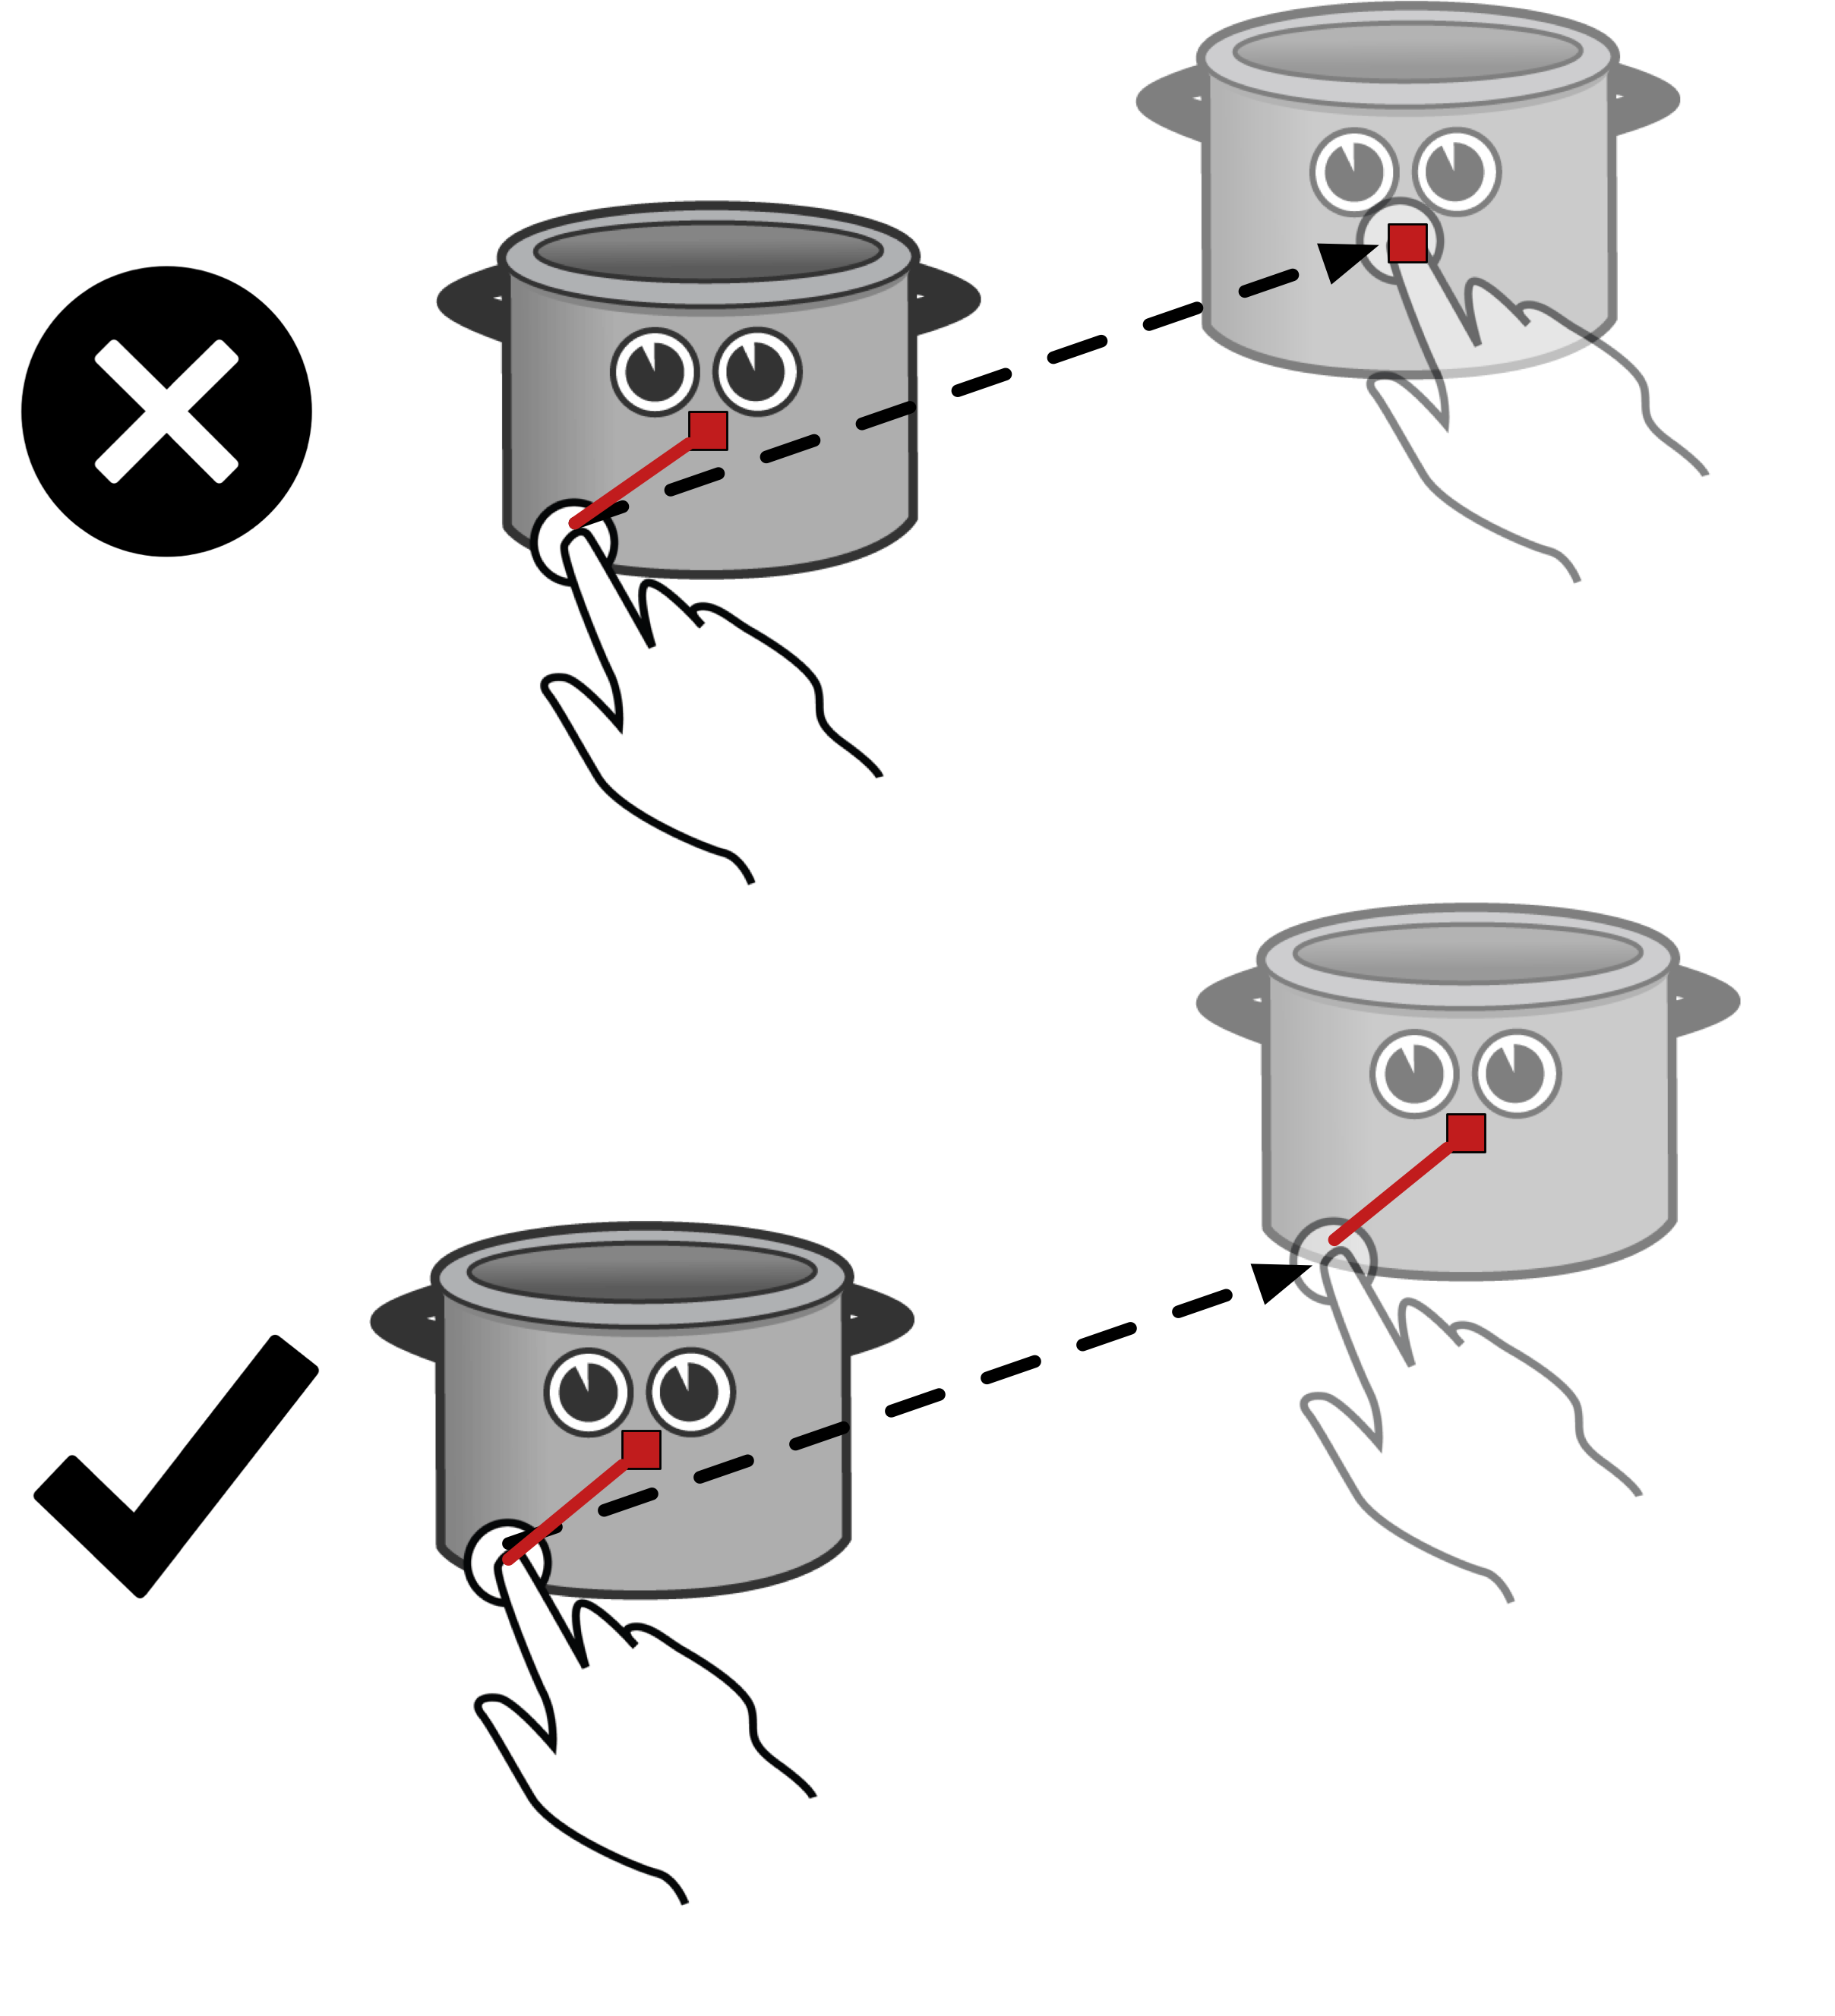
\includegraphics[width=0.4\linewidth]{images/Chapter3/dragging_offset.png}
		\caption{\textit{Top Image:} incorrect implementation, object jumps to touch
		position. \textit{Bottom Image:} correct implementation, touch offset is
		maintained while dragging the object.}
		\label{user_interaction_touch_offset}
\end{figure}
As the user moves the finger, we move the object along. However, the position of
the object is not exactly the touch position. Instead it is the touch position
\textit{plus} the touch offset determined when we started dragging. We determine
that offset by calculating the distance between the anchor point (that's the
reference point for positioning a node, typically it's in the center of the
node) of the touched object and the exact touch position. We calculate that
distance by subtracting the touch location from the anchor point location using
the \inlinecode{ccpSub} function. 

Now we know why it is important to store the touch offset!

\begin{leftbar}
To wrap up the implementation of \inlinecode{touchBegan} let's add the two
properties we have referenced: \inlinecode{isDraggingPot} and
\inlinecode{dragTouchOffset}. Your list of properties should now look like this:
\begin{lstlisting}
  weak var pot: CCSprite!
  
  private var fallingObjects = [FallingObject]()
  private let fallingSpeed = 100.0
  private let spawnFrequency = 0.5}
  (*@\colorbox{light-gray}{private var isDraggingPot = false}@*)
  (*@\colorbox{light-gray}{private var dragTouchOffset = ccp(0,0)}@*) 
\end{lstlisting}
\end{leftbar}

\subsection{Moving an Object}
Now we'll implement the code that actually moves the pot. That code needs to run
whenever a user's finger moves. That means we need to implement the
\inlinecode{touchMoved} method.
\begin{leftbar}
Add the \inlinecode{touchMoved} method below the \inlinecode{touchBegan} method:
\begin{lstlisting}
  override func touchMoved(touch: CCTouch, withEvent event: CCTouchEvent) {
    if (!isDraggingPot) {
      return
    }
    
    var newPosition = touch.locationInNode(self)
    // apply touch offset
    newPosition = ccpAdd(newPosition, dragTouchOffset);
    // ensure constant y position
    newPosition = ccp(newPosition.x, pot.positionInPoints.y);
    // apply new position to pot
    pot.positionInPoints = newPosition;
  }
\end{lstlisting}
\end{leftbar}
In the first line we check if we are currently in dragging mode. If not, we do
nothing and return immediately. This prevents the pot from jumping to the latest
touch position if it has not been picked up beforehand.

If we are in dragging mode we continue. First we get the new touch position.
Then we apply the offset that we discussed in figure
\ref{user_interaction_touch_offset} to that new position. The next line ensures
that the y position of the pot stays constant, we want to allow horizontal
movement only. Finally, we apply that new position to both pot parts. 

Great, we're pretty close to finishing the drag and drop functionality. If you
test the app in the current state you'll might see that there's one simple yet
important step missing\ldots

\subsection{Dropping an Object}
Right, the user will also want to drop the pot by releasing the finger from the
screen. 

Otherwise we stay in dragging mode forever and the pot will keep jumping
to whichever position the user taps on the screen. That kind of teleporting
would turn this game into a very simple one!

Luckily this can be easily implemented. All we need to do is to set
\inlinecode{isDraggingPot} to false as soon as the user stops touching the
screen.
\begin{leftbar}
Add the \inlinecode{touchEnded} method below the \inlinecode{touchMoved} method:
\begin{lstlisting}
  override func touchEnded(touch: CCTouch, withEvent event: CCTouchEvent) {
    isDraggingPot = false
  }
\end{lstlisting}
\end{leftbar}
Awesome! Our drag and drop code is complete! 

\section{Summary} 
Throughout this chapter you have implemented a drag and drop mechanism, while
learning more details about the \cocos{} touch system. Drag and drop mechanisms
can be used in many types of games, so what you have learned in this chapter is very valuable.

Now we can move on to the next chapter. We will implement one of the core
mechanics of our game - catching objects. In the next chapter you'll also learn
some interesting tricks and details about scene graphs and node transforms.

\subsection{Grab the Source Code}
You can find the Source Code for this chapter on GitHub:
\url{https://github.com/SpriteBuilder-Book/Code/tree/master/Chapter4/}.